\section{Monoscopic Reconstruction}
\label{sec:mono}

% The performance of the models trained with the previously mentioned setup,
% can be gauged by looking at the 
% figures \ref{fig:disp_test_perf} for the diffuse test set and 
% \ref{fig:disp_gamma_perf} for the performance on the 
% pointlike data. For the DISP regressor model,
% the R2 score is chosen as a measure for performance. In the case of the SIGN classification model, it is
% the accuracy.

% In both cases, it can be noted, that the DISP-model gets rapidly more
% powerful with higher energies up until ~\SI{1}{\tera\electronvolt}. From 
% thereon, the performance does not improve anymore and in fact seems to decline
% again. For the diffuse test set, an additional dip around \SI{3}{\tera\electronvolt}
% up to \SI{70}{\tera\electronvolt} can be made out, that cannot
% be explained at this point.
% For pointlike gamma events the performance seems to decrease less at high energies.
% It does however hit a peak at $\SI{10}{\tera\electronvolt}$.

% The SIGN-model does not saturate early and improves up to the highest energies,
% apart from the very last bin.

% For both model, the performance on the pointlike data is generally better.
% This is expected as
% the sensitiviy is best in the middle of the camera.

% \begin{figure}
%     \centering
%     \captionsetup{width=0.9\linewidth}
%     \begin{subfigure}{0.45\textwidth}
%         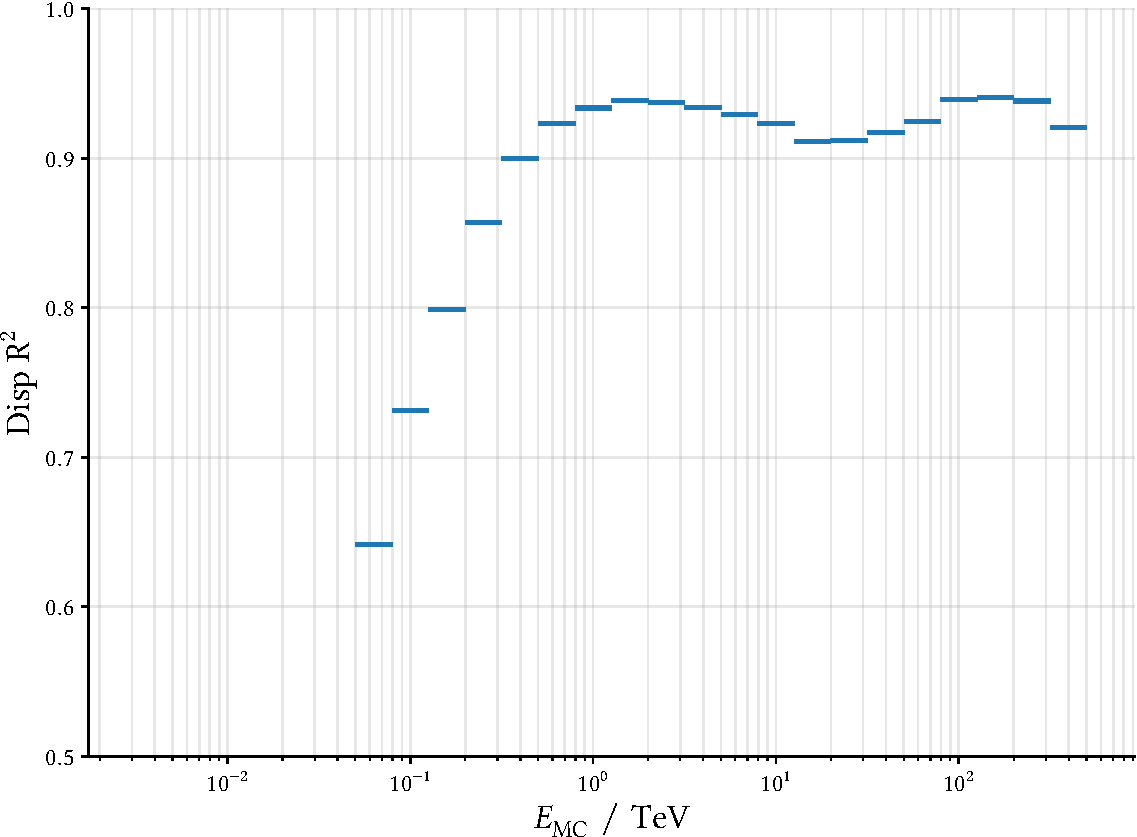
\includegraphics[width=\linewidth]{../analysis/plots/disp_test_r2_equal_sized.pdf} 
%         \caption{R2-Score for the DISP-estimation}
%     \end{subfigure}
%     \begin{subfigure}{0.45\textwidth}
%         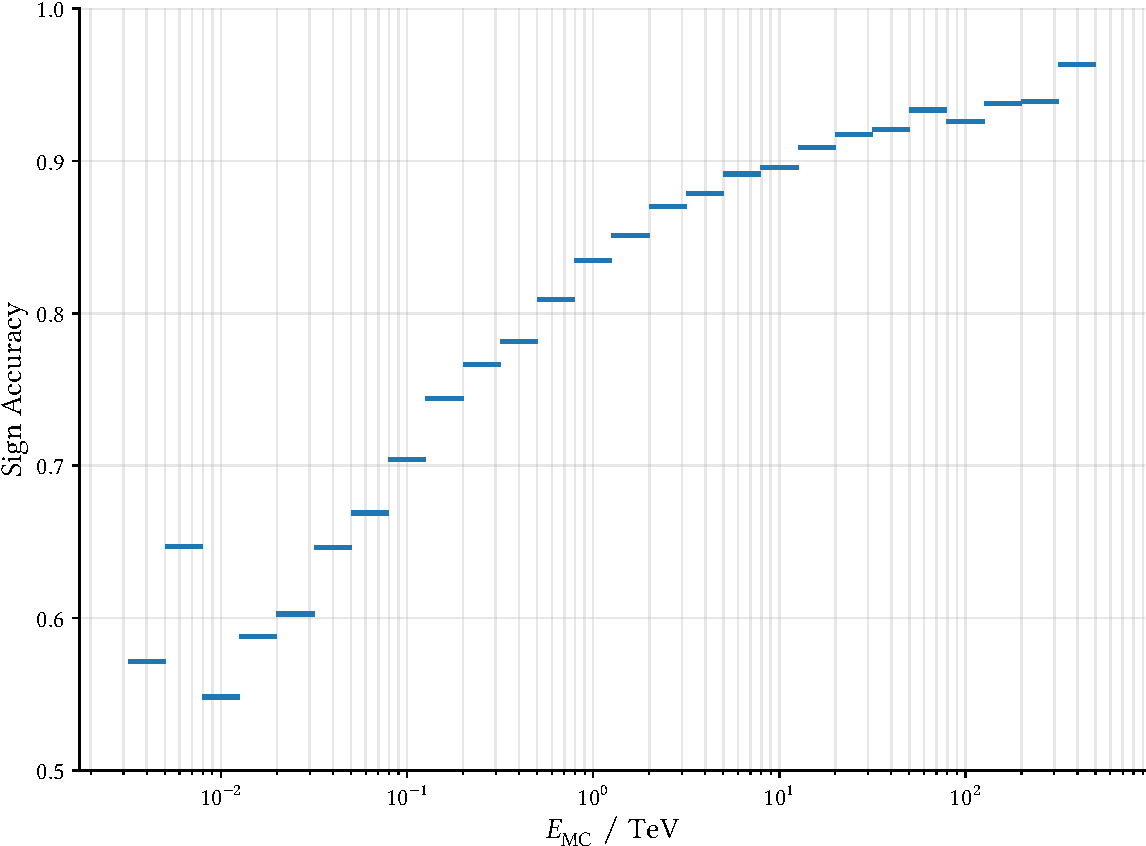
\includegraphics[width=\linewidth]{../analysis/plots/disp_test_acc_equal_sized.pdf}
%         \caption{Accuracy for the SIGN-estimation}
%     \end{subfigure}
%     \caption{
%     	Performance of the DISP- and SIGN-estimation algorithm on the diffuse test-dataset.
% 	Both model predictions improve with higher energies and saturate
% 	at $\approx\num{0.95}$ for the $R2$ and accuracy respectively.
%     The DISP-performance shows a dip in the energy range of \SI{3}{\tera\electronvolt}
%     up to \SI{70}{\tera\electronvolt}.}
%     \label{fig:disp_test_perf}
% \end{figure}

% \begin{figure}
%     \centering
%     \captionsetup{width=0.9\linewidth}
%     \begin{subfigure}{0.45\textwidth}
%         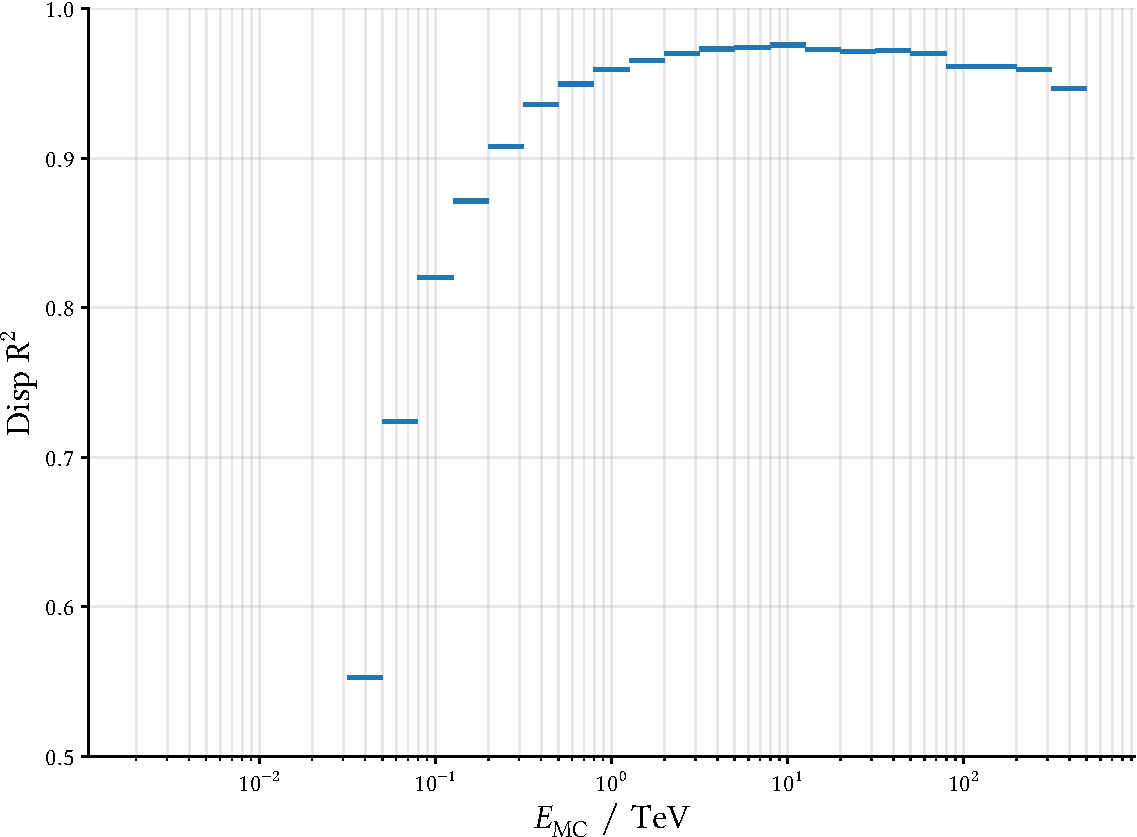
\includegraphics[width=\linewidth]{../analysis/plots/disp_gamma_r2_equal_sized.pdf} 
%         \caption{R2-Score for the DISP-estimation}
%     \end{subfigure}
%     \begin{subfigure}{0.45\textwidth}
%         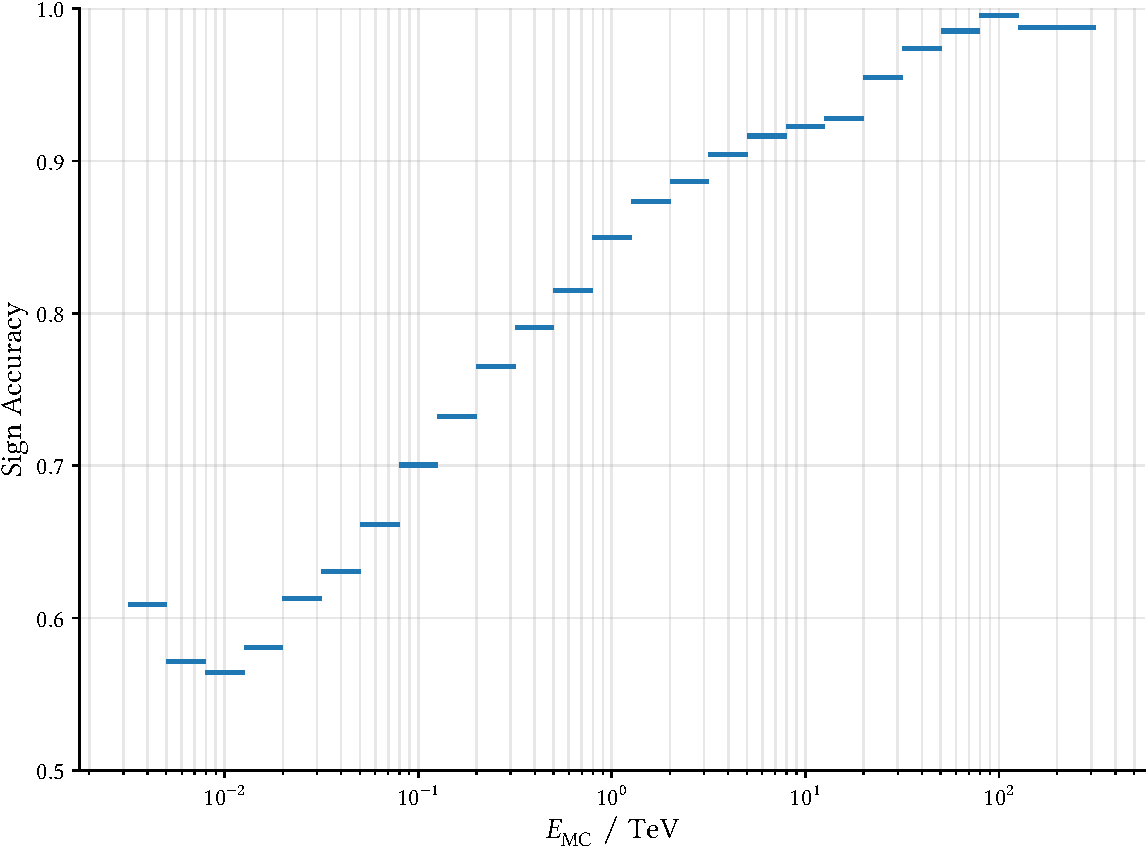
\includegraphics[width=\linewidth]{../analysis/plots/disp_gamma_acc_equal_sized.pdf}
%         \caption{SIGN-accuracy}
%     \end{subfigure}
%     \caption{
% 	Performance of the DISP- and SIGN-estimation algorithm on the pointlike dataset.
%     The R2-score of the DISP predictions shows a different form on pointlike
% 	compared to diffuse gammas: The performance generally is a bit better, 
% 	with saturation closer to 1. The dip at \SI{7}{\tera\electronvolt} is gone, but the highest energy bins
% 	show a decreasing performance.
%     The SIGN model performs similar, but the performance is slightly better throughout most of the energy range.}
%     \label{fig:disp_gamma_perf}
% \end{figure}
For the monoscopic reconstruction, all telescope events are taken as independent events and
the source position gets reconstructed using the DISP and SIGN model using the
pointlike gamma events.
Because events with misclasified SIGNs lead to predictions far away
from an assumed source position in a point source analysis of real data,
it can be argued to only keep events with properly reconstructed SIGNs.
In a real analysis, this would happen indirectly by performing a cut on 
the distance between assumed source position and reconstructed position.
On monte carlo data, we can just remove the events with misreconstructed SIGNs.
The angular resolution gets thus calculated with all reconstructed events and only with
the correctly reconstructed SIGNs.
This lowers the number of observed signal events,
but improves the angular resolution by a large margin.
Using only correctly assigned SIGNs on the pointlike dataset leaves 79\% of the events.
A sensitivity optimisation is not performed.

The angular resolution for all events
can be seen in figure \ref{fig:sens_telescope_gamma}.
Figure \ref{fig:sens_telescope_gamma_signs} shows only events with properly reconstructed SIGNs.
One can derive - in accordance to the previously discussed metrics - 
that both the DISP and SIGN predictions improve with increasing energies.
The predictions get worse at around the energies, where the $R2$-score
of the DISP-predictions saturates and decays.
Misreconstructed SIGNs are a problem expecially at low event energies as would be
expected from the accuracy of the SIGN model on the diffuse data.


% \begin{figure}
%     \centering
%     \captionsetup{width=0.9\linewidth}
%     \begin{subfigure}{0.45\textwidth}
%         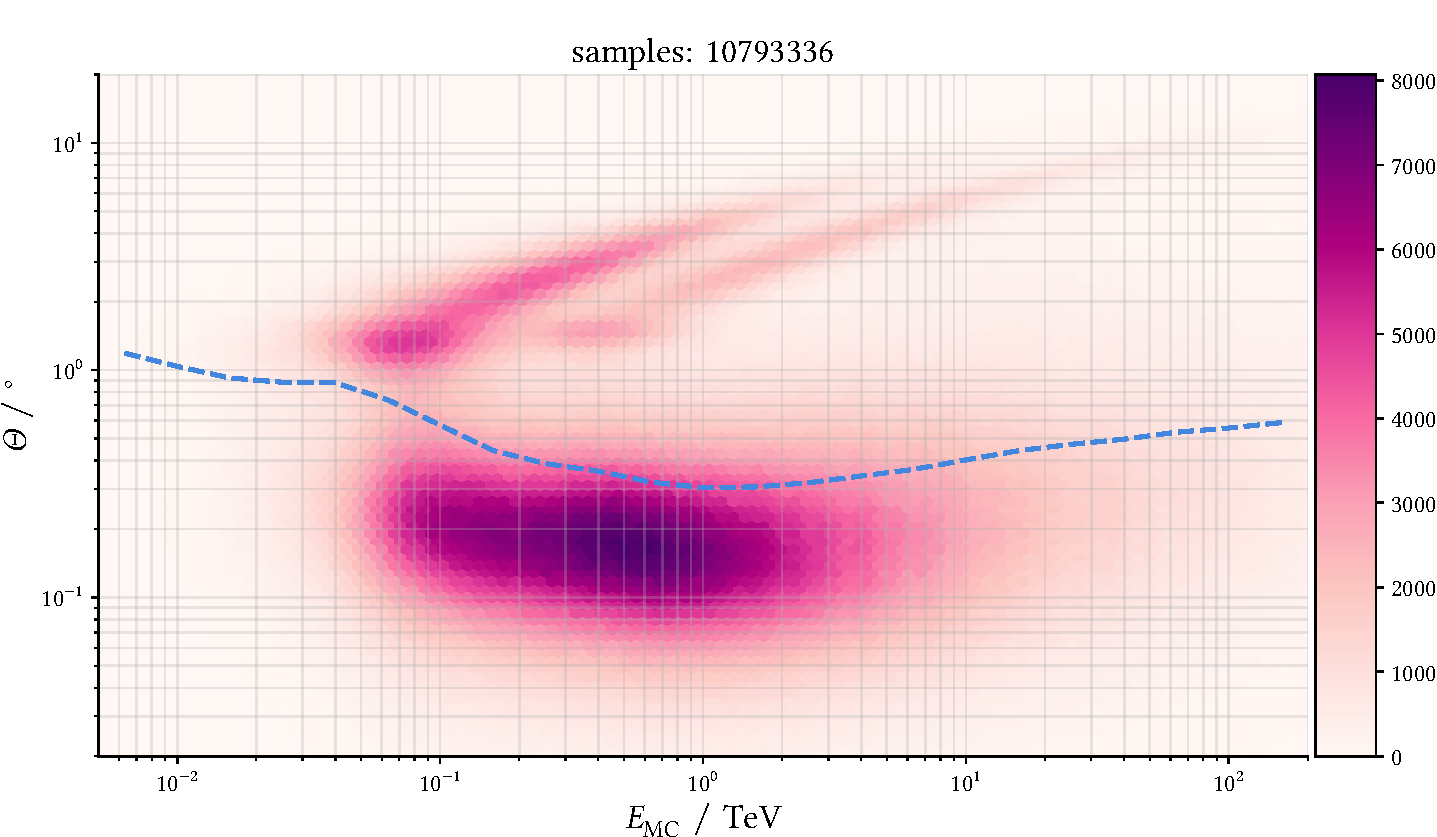
\includegraphics[width=0.6\textwidth]{../analysis/plots/test/tel_vs_energy.pdf}
%         \caption{All events}
%     \end{subfigure}
%     \begin{subfigure}{0.45\textwidth}
%         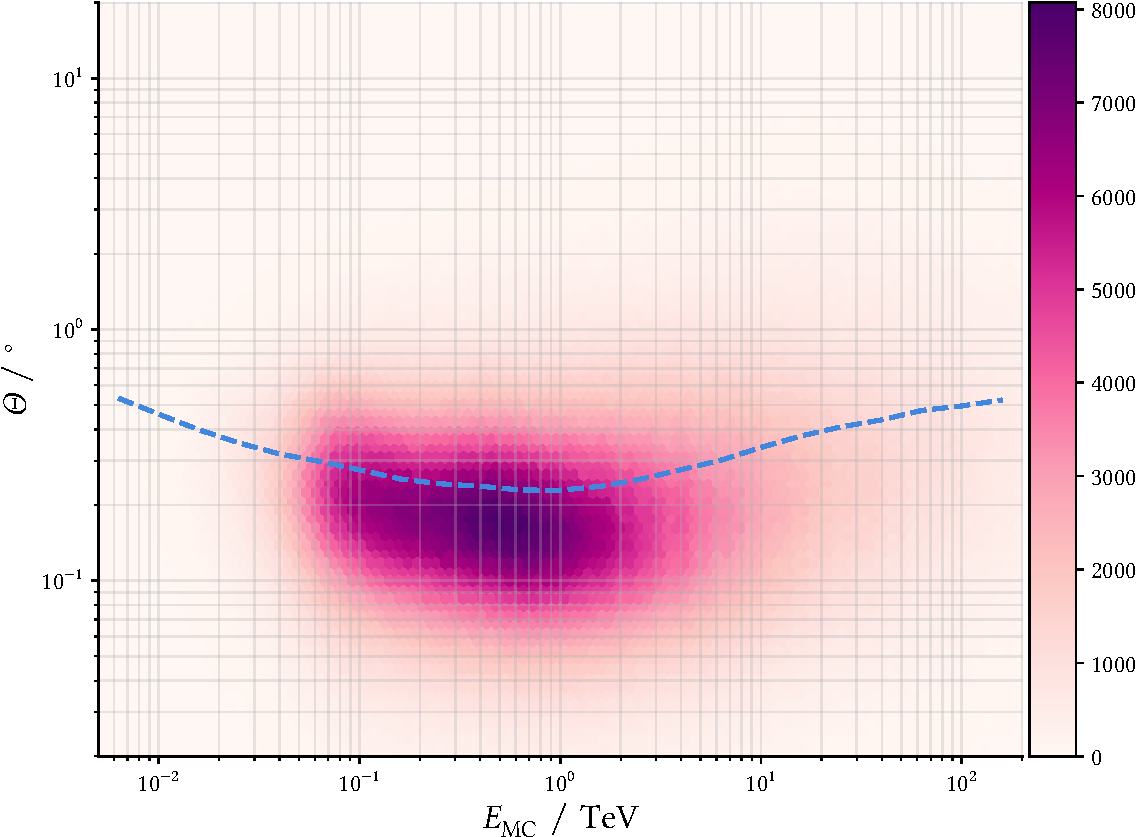
\includegraphics[width=0.6\textwidth]{../analysis/plots/test/tel_vs_energy_correct_signs.pdf}
%         \caption{Only correct SIGNs}
%     \end{subfigure}
%     \caption{
%         Monoscopic predictions for the source position on the pointlike 
%         test dataset with a total of XXX events. The blue-dotted line shows the 68\% containment. 
%         For lower energies, a big share of events has misreconstructed SIGNs,
%         leading to a second distribution with large $\Theta$. Upon removal of
%         the misclassified SIGNs, the 68\% containment on the
%         remaining XX events or XX\% is much improved.}
%     \label{fig:sens_telescope_test}
% \end{figure}

\begin{figure}
    \centering
    \captionsetup{width=0.9\linewidth}
    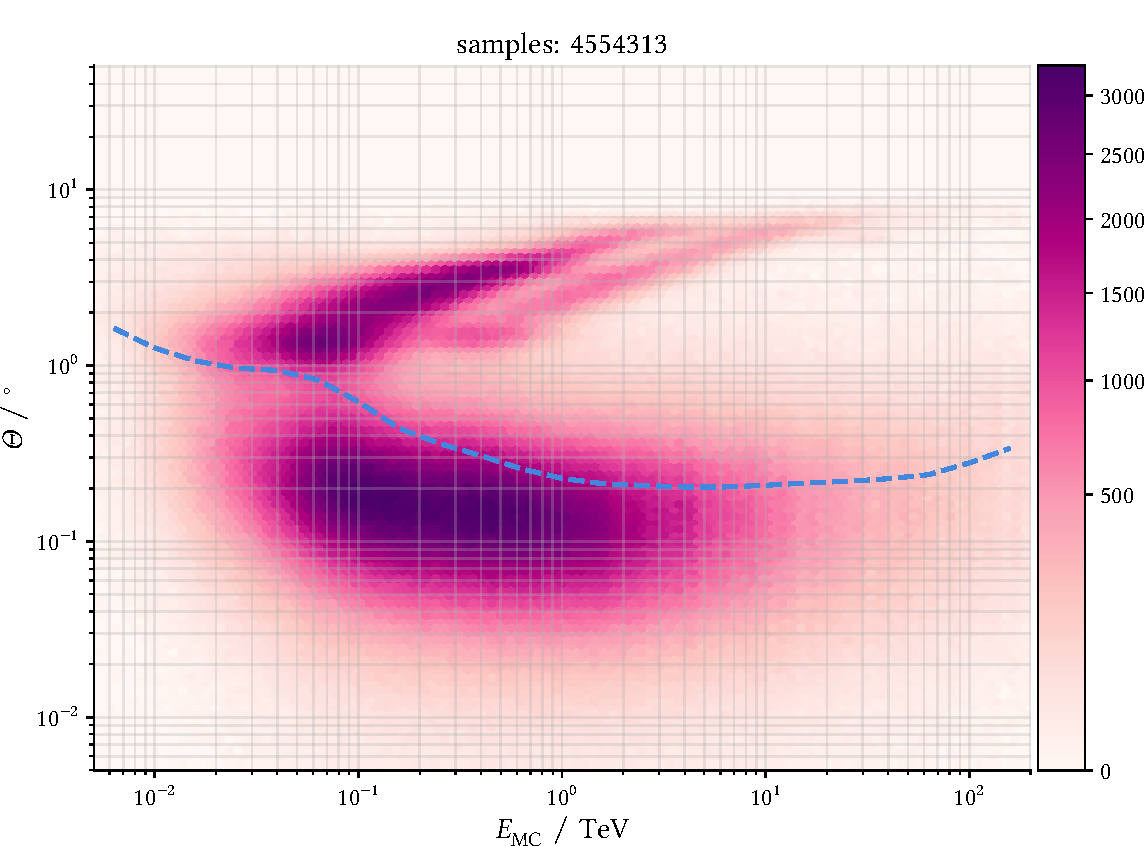
\includegraphics[width=0.6\textwidth]{../analysis/plots/gamma/tel_vs_energy.pdf}
    \caption{
        Monoscopic predictions for the source position on the pointlike 
        test dataset with a total of 4554313 telescope events.
        The blue-dotted line shows the 68\% containment. 
        For lower energies, a big share of events has misreconstructed SIGNs,
        leading to a second distribution with large $\Theta$.}
    \label{fig:sens_telescope_gamma}
\end{figure}


\begin{figure}
    \centering
    \captionsetup{width=0.9\linewidth}
    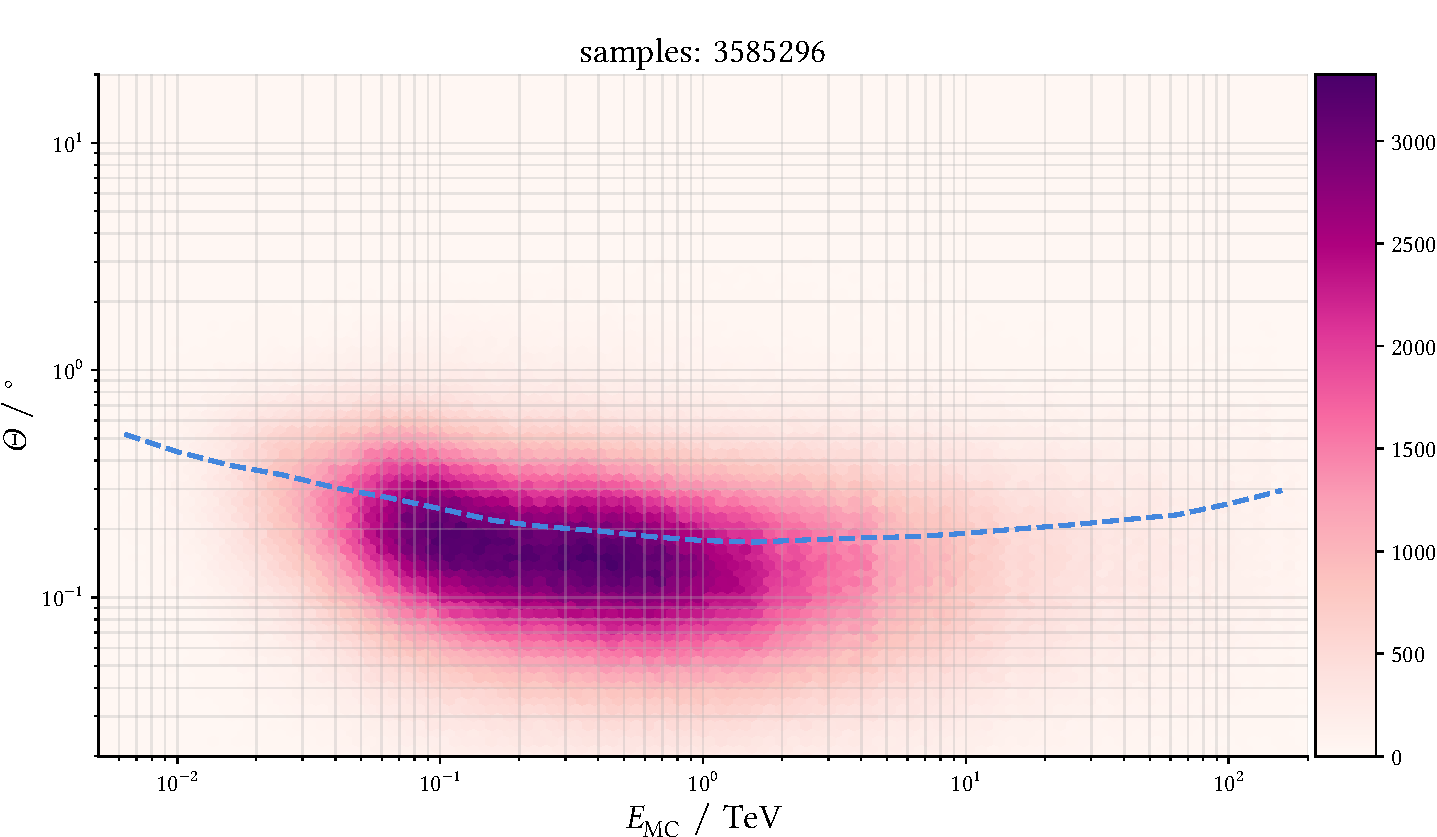
\includegraphics[width=0.6\textwidth]{../analysis/plots/gamma/tel_vs_energy_correct_signs.pdf}
    \caption{
        Monoscopic predictions for the source position on the pointlike 
        test dataset with a total of 3597952 events with properly reconstructed SIGNs. 
        The blue-dotted line shows the 68\% containment. 
        The angular resolution is much improved especially in the low energy regime
        where lots of events are removed.}
    \label{fig:sens_telescope_gamma_signs}
\end{figure}

% The feature importances for the DISP model can be seen in figure \ref{fig:disp_features},
% the one for the SIGN model in figure \ref{fig:sign_features}.
% For the DISP-model the reconstructed interaction heigth and core position
% show the most impact alongside the features, that describe the light content of
% the shower ellipse. The $length$ provides a lot of information whereas the
% $width$ is of little relevance for the prediction.
% The SIGN-predictions on the other hand are dominated by the observed 
% timing parameters $skewness$ and $slope$.

% \begin{figure}
% 	\centering
%     \captionsetup{width=0.9\linewidth}
% 	\hspace*{-0.15\textwidth}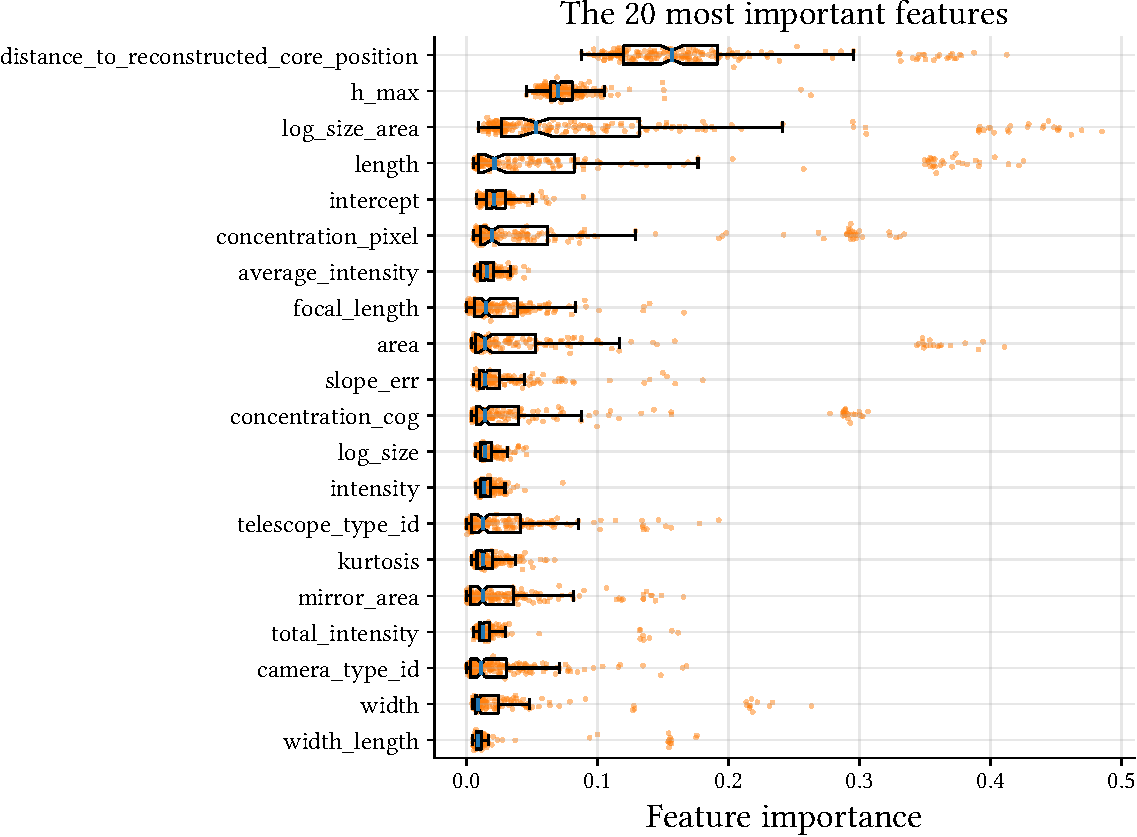
\includegraphics[width=0.6\textwidth]{../analysis/plots/disp_features.pdf}
% 	\caption{
% 	    Feature importance of the random forest for the DISP model.
% 	    The stereoscopic features have high influence on the prediction.
%     	From the monoscopic features, the features describing the light content and the
%         shape of the ellipse, provide most information.
%         Looking at the distribution of the individual feature importances, it 
%         can be derived that the range of important featrues is bigger than this list
%         with especially the $concentration$-features, the $area$, $width$ and $length$
%         being of high importance to the model as well.}
% 	\label{fig:disp_features}
% \end{figure}

% \begin{figure}
% 	\centering
%     \captionsetup{width=0.9\linewidth}
% 	\hspace*{-0.15\textwidth}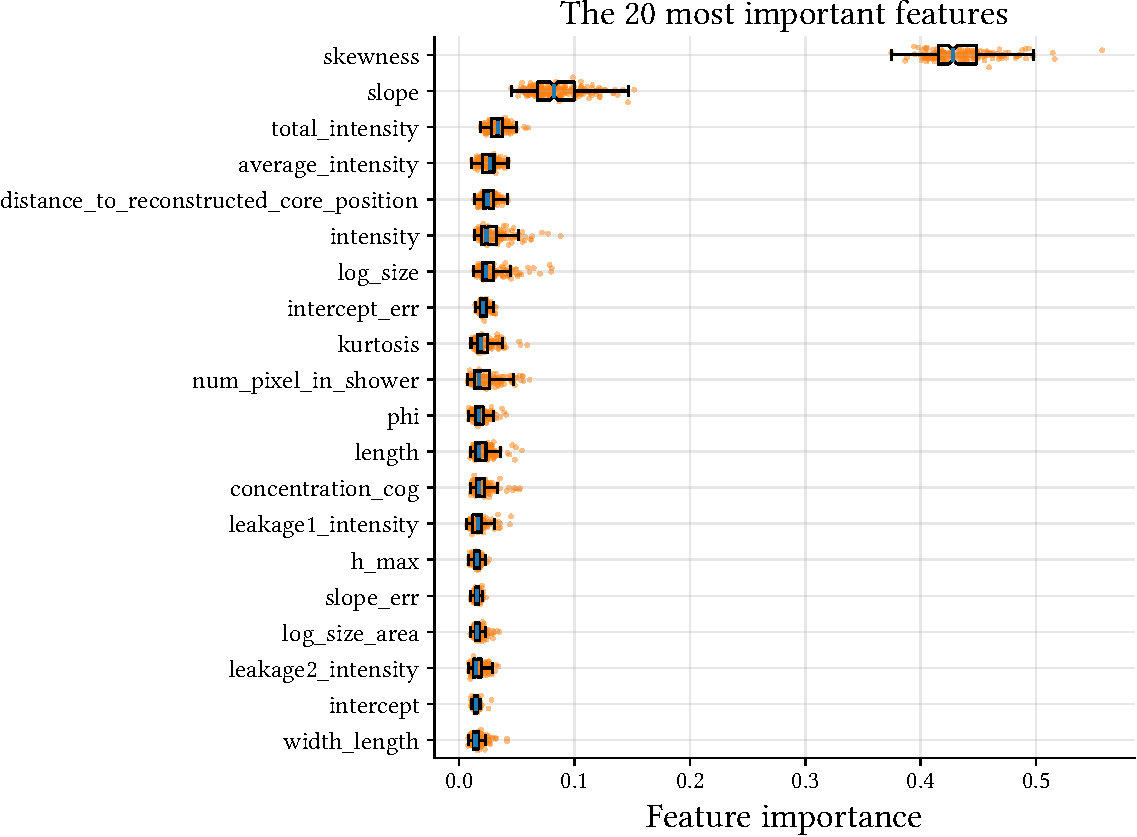
\includegraphics[width=0.6\textwidth]{../analysis/plots/sign_features.pdf}
% 	\caption{Feature importance of the random forest for the SIGN model.
% 	        The most influential features to the prediction are by far the higher-order moments $skewness$
%             and $slope$. The stereoscopic features do not provide much information,
%             which is expected as the head-/tail-ambiguation is entirely an artefact produced
%             in the camera frame. Other features provide very little information.}
% 	\label{fig:sign_features}
% \end{figure}


\section{Stereoscopic Reconstruction}\label{position}

Using the models mentioned in \ref{sec:mono}, the resulting DISP+SIGN predictions
are combined transforming the predictions to the nominal frame and then
transforming the median in the nominal frame to the horizon frame.
The angular resolution over the true event energy of this baseline stereoscopic predictions
compared to the existing HillasReconstructor can be seen in figure \ref{fig:stereo_median_energy}.
The angular resolution against the event multiplicity is displayed in figure \ref{fig:stereo_median_multi}.

At each energy, the HillasReconstructor performs considerably better.
One can derive that the median predictions do not improve considerably above
\SI{3}{\tera\electronvolt} and get worse above \SI{10}{\tera\electronvolt}.
The HillasReconstructor shows a saturation at the highest energies,
but without the prominently decaying performance of the median predictions.
It can also be noted, that the median predictions seem to not completely
resolve the problem with wrong SIGNs.

Looking at the performance over the event multiplicity we can conclude that the median predictions
do not scale as well with higher multiplicities, so that the performance gap increases with
the multiplicities going up.

The HillasReconstructor also shows a pronounced bump in the range of \SI{200}{\giga\electronvolt}
to \SI{1}{\tera\electronvolt}. 
This can be connected to a high number of low multiplicity events in the
LST-MST crossover region, which limits the performance.
% This has been observed in other analyses as well and seems to correlate with 
% a lot of low multiplicity events in the crossover region from LSTs to MSTs \cite{kai? max?}.

\begin{figure}
    \centering
    \captionsetup{width=0.9\linewidth}
    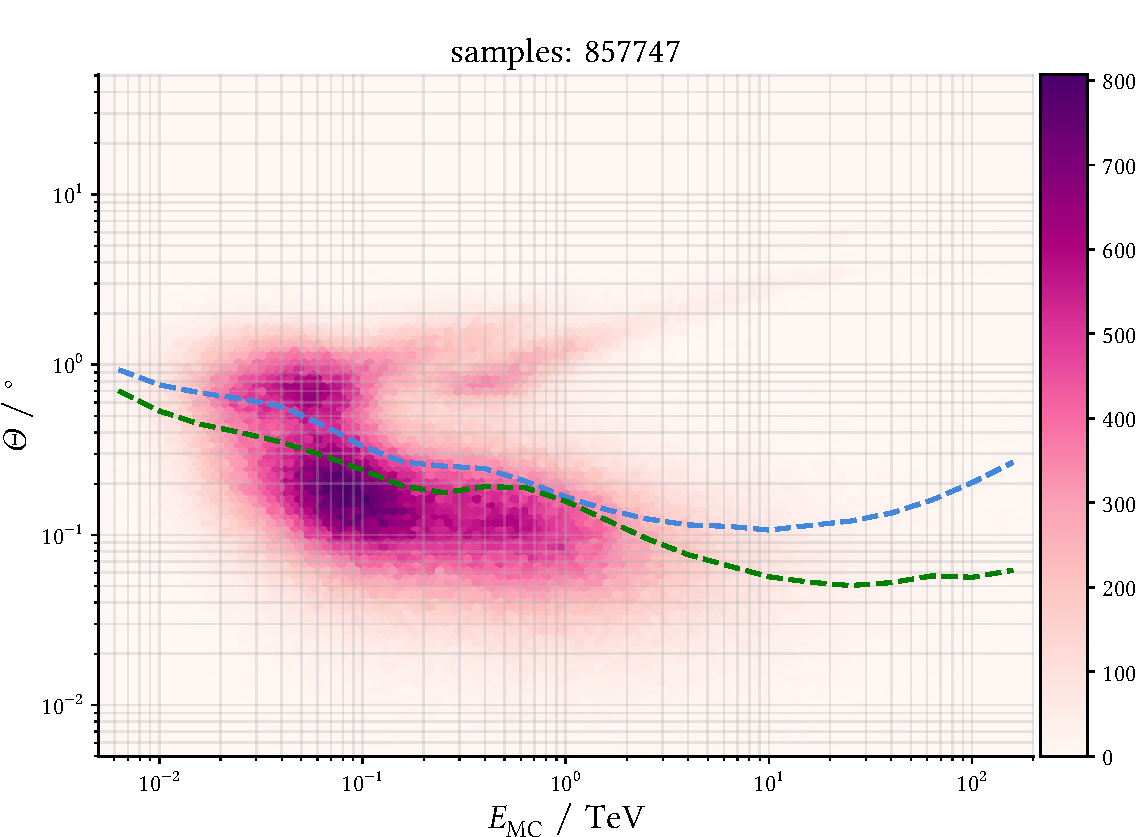
\includegraphics[width=0.6\textwidth]{../analysis/plots/gamma/median_vs_energy.pdf} 
    \caption{Distance between predicted and true position over true energy as obtained by taking the median of
    the DISP+SIGN predictions on 955317 pointlike gamma events. The blue line shows the 
    68\% containment of these results. The green line refers to the 68\%
    results of the HillasReconstructor, which is added for comparison, but has no
    connection to the binned results.
    Despite the short bump in the range of \SI{200}{\giga\electronvolt}
    to \SI{1}{\tera\electronvolt} the HillasReconstructor outperforms the median predictions
    massively.}
    \label{fig:stereo_median_energy}
\end{figure}

\begin{figure}
    \centering
    \captionsetup{width=0.9\linewidth}
    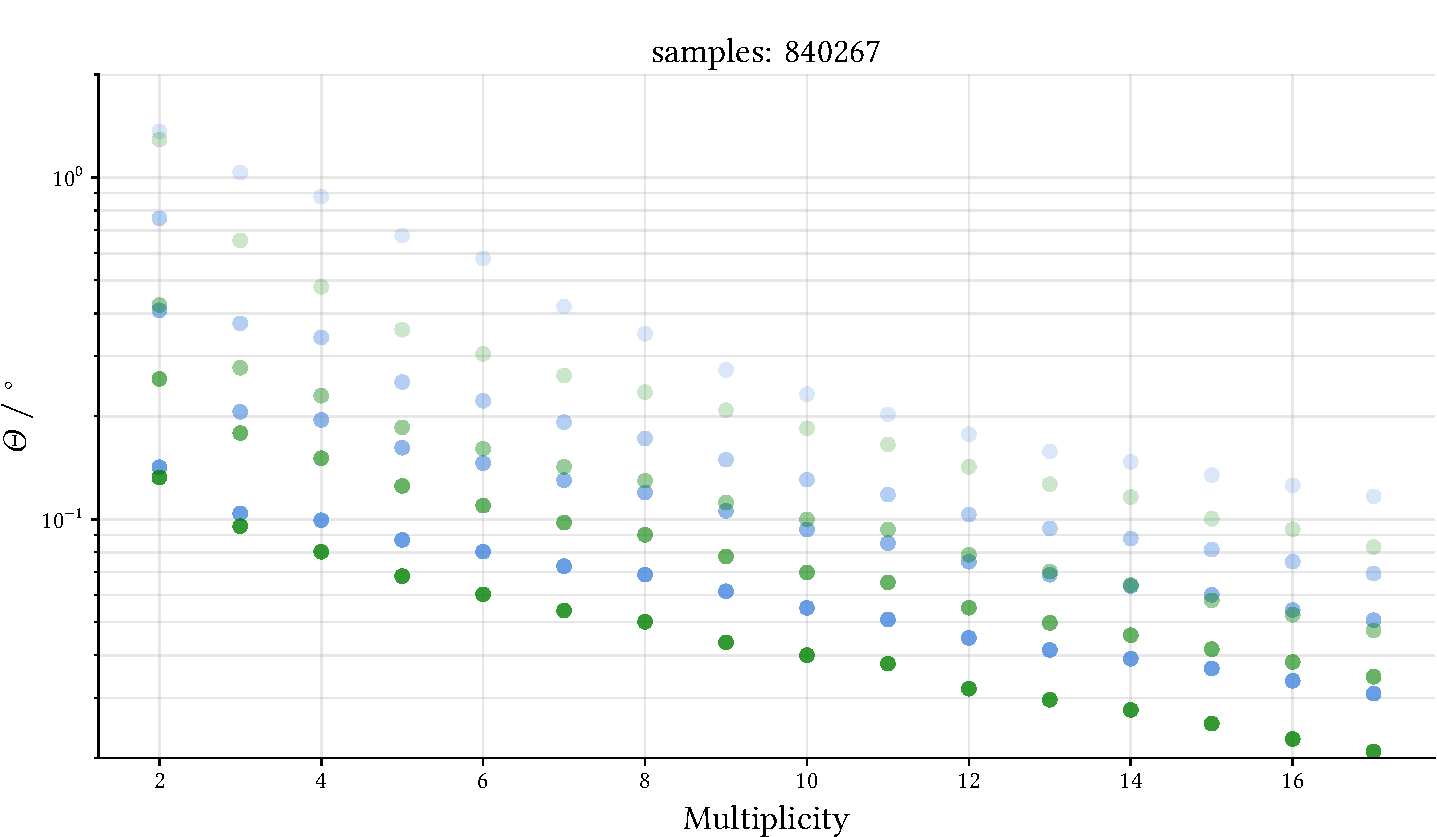
\includegraphics[width=0.6\textwidth]{../analysis/plots/gamma/median_vs_multi_comp.pdf}
    \caption{Distance between predicted and true position over event multiplicity as obtained by taking
    the median, if the DISP+SIGN predictions (blue) and using the HillasReconstructor (green)
    on 955317 pointlike gamma events. 
    The different dots refer to the 25, 50, 68 and 90\% percentiles with 
    lowering opacity.
    The median predictions are worse at every multiplicity and the gap increases with higher event multiplicity.}
    \label{fig:stereo_median_multi}
\end{figure}

The results of the iterative DISP-approach can be seen in figures
\ref{fig:stereo_magic_energy} and \ref{fig:stereo_magic_multi}.
Compared to the median predictions, the 68\% percentile is much improved throughout the complete energy range besides 
the very highest energies. At this point the error of the DISP-predictions is probably limiting and the 
HillasReconstructor leads to much better results.
At the lower energy range the approach seems to be working well, outperforming the HillasReconstructor.

When looking at the multiplicity dependency, we see improved results as well. 
At high event multiplicities the Hillas-reconstructor still
leads to better results. At low multiplicites on the other hand,
especially at 2- and 3-multiplicity events, the apporach works very well.
The HillasReconstructor starts to outperform at multiplicities of 4-6.

\begin{figure}
    \centering
    \captionsetup{width=0.9\linewidth}
    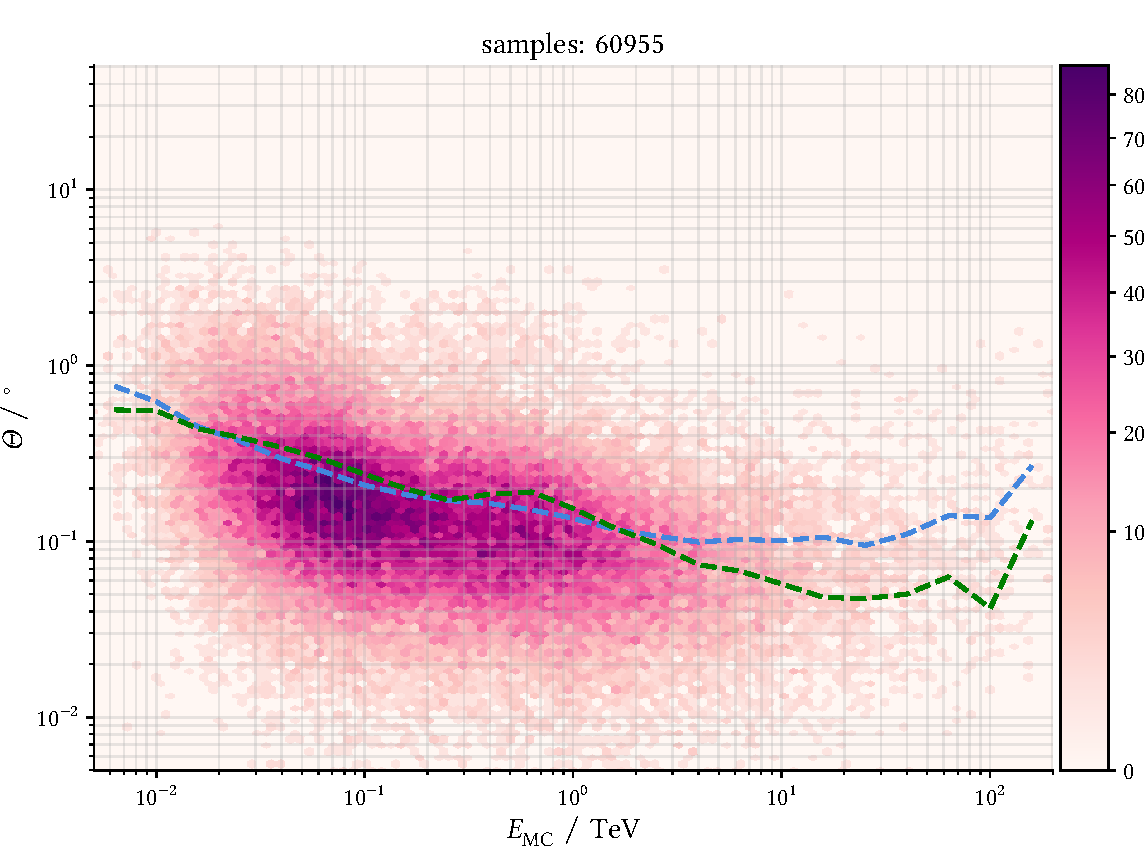
\includegraphics[width=0.6\linewidth]{../analysis/plots/gamma/pairwise_median_100_vs_energy.pdf} 
    \caption{Distance between predicted and true position over true event energy as obtained with the
    iterative DISP approach on 955317 pointlike gamma events.
    The binned results refer to the iterative DISP-predictions. The blue line shows the 
    68\% containment of these results. The green line refers to the 68\%
    results of the HillasReconstructor.
    The DISP-approach outperforms the HillasReconstructor up to
    $\approx \SI{2}{\tera\electronvolt}$.}
    \label{fig:stereo_magic_energy}
\end{figure}

\begin{figure}
    \centering
    \captionsetup{width=0.9\linewidth}
    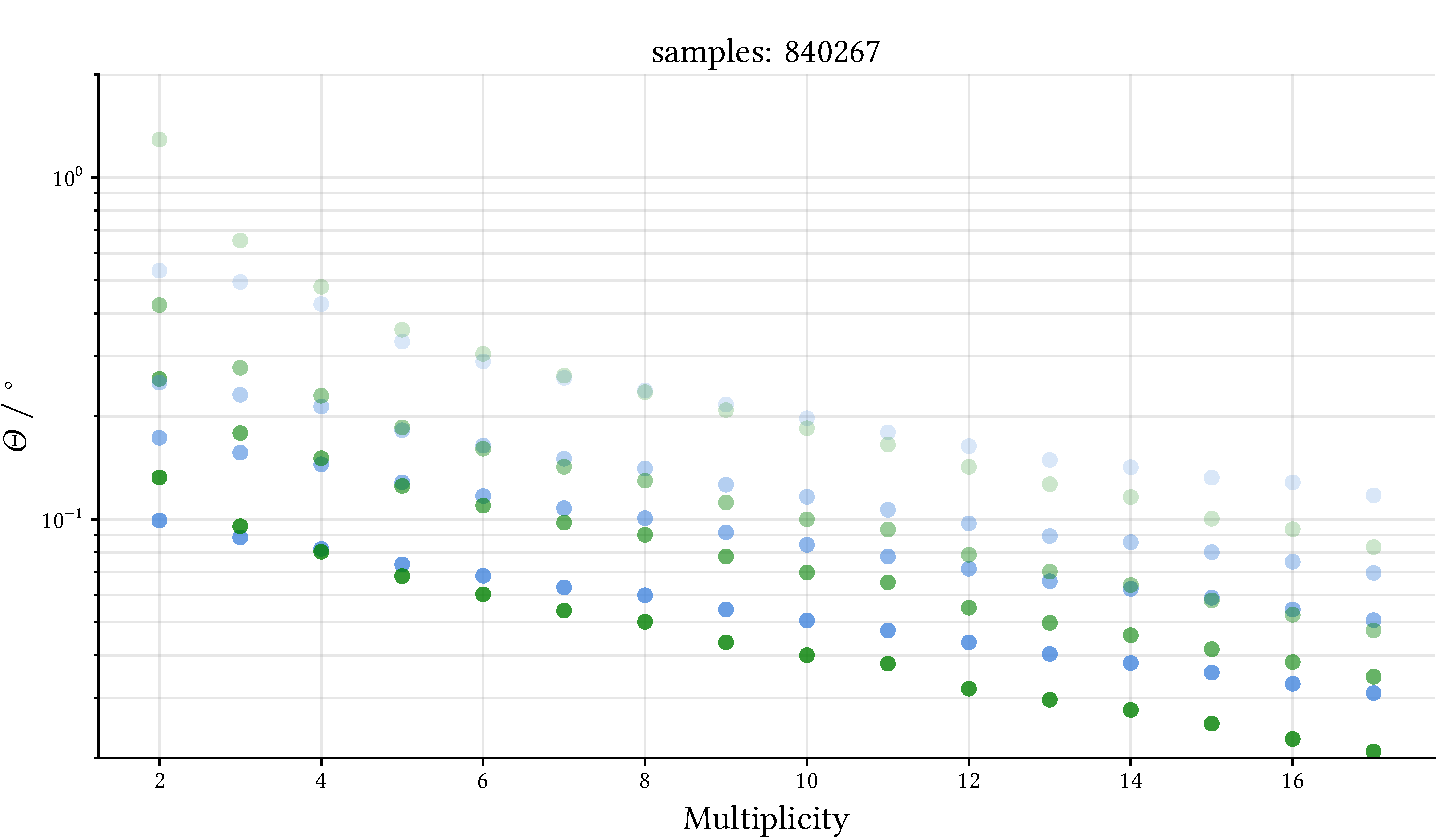
\includegraphics[width=0.6\linewidth]{../analysis/plots/gamma/pairwise_median_100_vs_multi_comp.pdf}
    \caption{Distance between predicted and true position over event multiplicity as obtained with
    the iterative DISP approach (blue) and the HillasReconstructor (green)
    on 955317 pointlike gamma events.
    The different lines refer to the 25,50,68 and 90\% percentiles with 
    lowering opacities.
    For low multiplicities, the combined DISP-predictions are superiour, 
    for high multiplicities the HillasReconstructor results win out.
    The breakeven point seems to be at 4-6 telescopes, depending on 
    which percentiles have more weight to the analysis.}
    \label{fig:stereo_magic_multi}
\end{figure}

\section{Stereoscopic Sensitivities}

Two independent sensitivity optimisations are being performed,
one for the HillasReconstructor analysis and one for the stereoscopic DISP analysis.
The background separation and energy models are the same in both cases
as are the preprocessed datasets.
The pointlike gamma data acts as signal events, the background is formed by
the proton test set. The results get compared
to the CTA reference analysis \cite{cta_web}.
Details of the reference analysis have not been shared.
In this case it merely included as a naive benchmark, because
comparability can not be assumed.
For the same reason and with the same limitations
the CTA requrements are included as well.
Even If nothing else, the purely protonic background is a large simplification
and the background statistic in general seems to be too low to
provide proper sensitivities. 

Starting with the HillasReconstructor, the prediction
and theta cut get optimized in each bin of energy performing a gridsearch on the 
values of the event multiplicity, $\Theta$ and prediction threshold.
The possible range of values is:

$$ \Theta: 0.01, 0.02, \ldots, 0.17 $$
$$ \text{prediction threshold} \alpha: 0.5, 0.55, \ldots, 1.00 $$
$$ \text{multiplicity}: 2, 3, \ldots, 10 $$

Best sensitivities get achieved with the following parameter combination:

% \afterpage{
%     \thispagestyle{empty}
%     \begin{landscape}
%         %\caption{Optimized cuts for the Hillasreconstructor analysis in logarithmic energy bins.
%         %The event counts correspond to the counts after weighting.}
%         %\begin{center}
%             \centering
%             \begin{tabular}{c c c c c r c c}
%                 %\hline
%                 $E_\text{min}$ / \si{\tera\electronvolt} & $E_\text{max}$ / \si{\tera\electronvolt} & $\alpha$ & $\Theta$ & Mult. & Sign. & sig counts & bkg counts \\
%                 \hline
%                 \num{0.02} & \num{0.03} & 0.75 & 0.12 & 2 & \num{67.081609668104} & \num{12684.82} (\num{3119}) & \num{125557.82} (\num{476})\\
%                 \num{0.03} & \num{0.05} & 0.6 & 0.17 & 2 & \num{143.914706929475} & \num{58145.94} (\num{13840}) & \num{572791.75} (\num{1214}) \\
%                 \num{0.05} & \num{0.08} & 0.6 & 0.17 & 2 & \num{327.902927338685} & \num{166199.76} (\num{38918}) & \num{774710.40} (\num{2032}) \\
%                 \num{0.08} & \num{0.12} & 0.6 & 0.16 & 2 & \num{466.286269748645} & \num{160335.10} (\num{38495}) & \num{234553.03} (\num{852}) \\
%                 \num{0.13} & \num{0.20} & 0.7 & 0.11 & 6 & \num{404.026953731173} & \num{58324.53} (\num{14379}) & \num{9678.95} (\num{83}) \\
%                 \num{0.20} & \num{0.32} & 0.8 & 0.09 & 6 & \num{291.173501331132} & \num{24694.15} (\num{6922}) & \num{404.89} (\num{6}) \\
%                 \num{0.32} & \num{0.50} & 0.8 & 0.08 & 10 & \num{278.308880907216} & \num{21899.35} (\num{6949}) & \num{84.86} (\num{2}) \\
%                 \num{0.50} & \num{0.80} & 0.8 & 0.07 & 6 & \num{301.554242885264} & \num{25516.59} (\num{9771}) & \num{35.88} (\num{2}) \\
%                 \num{0.80} & \num{1.26} & 0.8 & 0.06 & 7 & \num{238.800568473337} & \num{16000.56} (\num{7552}) & \num{22.20} (\num{2}) \\
%                 \num{1.26} & \num{2.00} & 0.75 & 0.05 & 10 & \num{193.005662032815} & \num{10450.36} (\num{6207}) & \num{13.98} (\num{2}) \\
%                 \num{2.00} & \num{3.17} & 0.75 & 0.06 & 6 & \num{189.144224666632} & \num{10008.57} (\num{8098}) & \num{5.70} (\num{1}) \\
%                 \num{3.17} & \num{5.02} & 0.7 & 0.05 & 7 & \num{140.184997871284} & \num{5512.73} (\num{6114}) & \num{7.27} (\num{3}) \\
%                 \num{5.02} & \num{7.96} & 0.7 & 0.05 & 9 & \num{97.3831573129413} & \num{2656.42} (\num{4223}) & \num{2.40} (\num{1}) \\
%                 \num{7.96} & \num{12.62} & 0.7 & 0.06 & 6 & \num{79.3212652969814} & \num{1764.58} (\num{4219}) & \num{2.21} (\num{1}) \\
%                 \num{12.62} & \num{20.00} & 0.65 & 0.05 & 4 & \num{56.0187708296887} & \num{899.54} (\num{3306}) & \num{8.42} (\num{6}) \\
%                 \num{20.00} & \num{31.70} & 0.6 & 0.06 & 5 & \num{38.4920204879829} & \num{417.91} (\num{2431}) & \num{1.27} (\num{1}) \\
%                 \num{31.70} & \num{50.24} & 0.55 & 0.07 & 3 & \num{27.1123543279959} & \num{210.29} (\num{2063}) & \num{1.76} (\num{1}) \\
%                 \num{50.24} & \num{72.62} & 0.45 & 0.07 & 3 & \num{17.4720214115349} & \num{88.46} (\num{1526}) & \num{1.24} (\num{1}) \\
%                 \num{79.62} & \num{126.19} & 0.45 & 0.07 & 2 & \num{9.47422298618942} & \num{27.84} (\num{865}) & \num{1.45} (\num{2}) \\
%                 \num{126.19} & \num{200.00} & 0.35 & 0.17 & 2 & \num{3.52411688223802} & \num{10.01} (\num{578}) & \num{17.27} (\num{5}) \\
%             %\hline
%             \end{tabular}
%         %\end{center}
%         %\label{tab:hillas_cuts}
%     \end{landscape}
% }
% \clearpage


%\KOMAoptions{paper=landscape,pagesize}
%\recalctypearea
\newpage
\storeareas\normalsetting
\KOMAoption{paper}{landscape}
\areaset{4\textwidth}{.9\textheight}
\recalctypearea
    \centering
    %\captionsetup{width=0.9\linewidth}
    \captionof{table}{Thresholds, significances and event counts for the sensitivity curve of the
    HillasReconstructor analysis. The event counts related to the weighted events. The unweighted event counts are given
    in brackets behind.}
    \begin{tabular}{r r r r r r r r c }
        %\hline
        $E_\text{min}$ / \si{\tera\electronvolt} & $E_\text{max}$ / \si{\tera\electronvolt} & $\alpha$ & $\Theta$ & Multiplicity & Sign. &  \multicolumn{2}{| c |}{test} & Bkg Counts \\
        \hline
        \num{0.02} & \num{0.03} & 0.75 & 0.12 & 2 & \num{67.08} & \num{12684.82} & \num{3119} & \num{125557.82} (\num{476})\\
        \num{0.03} & \num{0.05} & 0.6 & 0.17 & 2 & \num{143.91} & \num{58145.94} & \num{13840} & \num{572791.75} (\num{1214}) \\
        \num{0.05} & \num{0.08} & 0.6 & 0.17 & 2 & \num{327.90} & \num{166199.76} & \num{38918} & \num{774710.40} (\num{2032}) \\
        \num{0.08} & \num{0.12} & 0.65 & 0.16 & 2 & \num{466.29} & \num{160335.10} & \num{38495} & \num{234553.03} (\num{852}) \\
        \num{0.13} & \num{0.20} & 0.7 & 0.11 & 6 & \num{404.03} & \num{58324.53} & \num{14379} & \num{9678.95} (\num{83}) \\
        \num{0.20} & \num{0.32} & 0.8 & 0.09 & 6 & \num{291.17} & \num{24694.15} & \num{6922} & \num{404.89} (\num{6}) \\
        \num{0.32} & \num{0.50} & 0.8 & 0.08 & 10 & \num{278.31} & \num{21899.35} & \num{6949} & \num{84.86} (\num{2}) \\
        \num{0.50} & \num{0.80} & 0.8 & 0.07 & 6 & \num{301.55} & \num{25516.59} & \num{9771} & \num{35.88} (\num{2}) \\
        \num{0.80} & \num{1.26} & 0.8 & 0.06 & 7 & \num{238.80} & \num{16000.56} & \num{7552} & \num{22.20} (\num{2}) \\
        \num{1.26} & \num{2.00} & 0.75 & 0.05 & 10 & \num{193.01} & \num{10450.36} & \num{6207} & \num{13.98} (\num{2}) \\
        \num{2.00} & \num{3.17} & 0.75 & 0.06 & 6 & \num{189.14} & \num{10008.57} & \num{8098} & \num{5.70} (\num{1}) \\
        \num{3.17} & \num{5.02} & 0.7 & 0.05 & 7 & \num{140.18} & \num{5512.73} & \num{6114} & \num{7.27} (\num{3}) \\
        \num{5.02} & \num{7.96} & 0.7 & 0.05 & 9 & \num{97.38} & \num{2656.42} & \num{4223} & \num{2.40} (\num{1}) \\
        \num{7.96} & \num{12.62} & 0.7 & 0.06 & 6 & \num{79.32} & \num{1764.58} & \num{4219} & \num{2.21} (\num{1}) \\
        \num{12.62} & \num{20.00} & 0.65 & 0.05 & 4 & \num{56.02} & \num{899.54} & \num{3306} & \num{8.42} (\num{6}) \\
        \num{20.00} & \num{31.70} & 0.6 & 0.06 & 5 & \num{38.49} & \num{417.91} & \num{2431} & \num{1.27} (\num{1}) \\
        \num{31.70} & \num{50.24} & 0.55 & 0.07 & 3 & \num{27.11} & \num{210.29} & \num{2063} & \num{1.76} (\num{1}) \\
        \num{50.24} & \num{72.62} & 0.45 & 0.07 & 3 & \num{17.47} & \num{88.46} & \num{1526} & \num{1.24} (\num{1}) \\
        \num{79.62} & \num{126.19} & 0.45 & 0.07 & 2 & \num{9.47} & \num{27.84} & \num{865} & \num{1.45} (\num{2}) \\
        \num{126.19} & \num{200.00} & 0.35 & 0.17 & 2 & \num{3.52} & \num{10.01} & \num{578} & \num{17.27} (\num{5}) \\
    %\hline
    \end{tabular}
    \label{tab:test}
\clearpage
\newpage
% \KOMAoptions{paper=portrait,pagesize}
% \recalctypearea
\normalsetting



The sensitivity curve is displayed in figure \ref{fig:hillas_sens}.

The results exceed the reference analysis albeit with relatively large uncertainties
at higher energies.

\begin{figure}
    \centering
    \captionsetup{width=0.9\linewidth}
    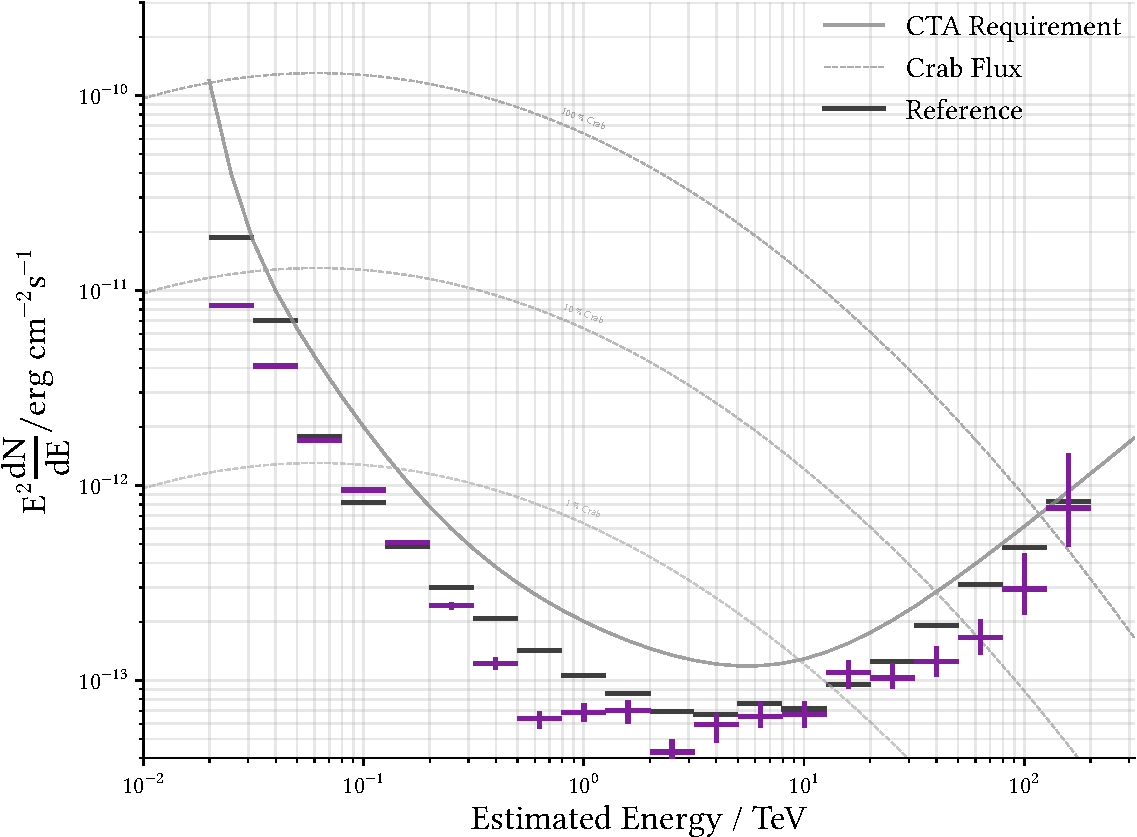
\includegraphics[width=0.6\textwidth]{../analysis/plots/sensitivity/hillas_sensitivity.pdf} 
    \caption{Computed sensitivity for the HillasReconstructor analysis against estimated event energy.
    The CTA requirements and
    reference results are added although a direct comparison is difficult. It can be noted though, that
    the general trend matches the expected results with the best sensitivity in the range from
    \num{1} to \SI{10}{\tera\electronvolt}. At high energies the uncertainties are increasing due to the low
    background statistic.}
    \label{fig:hillas_sens}
\end{figure}

With the cuts from the sensitivity optimisation, the effective area and angular resolution can be
compared as well.

The effective area, shown in figure \ref{fig:hillas_area}, exceeds the reference.
The angular resolution on the signal events, displayed in figure \ref{fig:hillas_resol}, is illustrated without
the $\Theta$ cuts to show the quaity of the reconstruction after apllying the
other cuts.
The large effective area is probably connected with the simplified background model
and the absence of cuts at lower data levels, such as on the number of pixels or
leakage, in this analysis.
At the same time the background counts in this analysis are already very low at high energies.
This leads to the conclusion, that the available statistic is just not sufficient
to get to any quantitative conclusions at high energies.

\begin{figure}
    \centering
    \captionsetup{width=0.9\linewidth}
    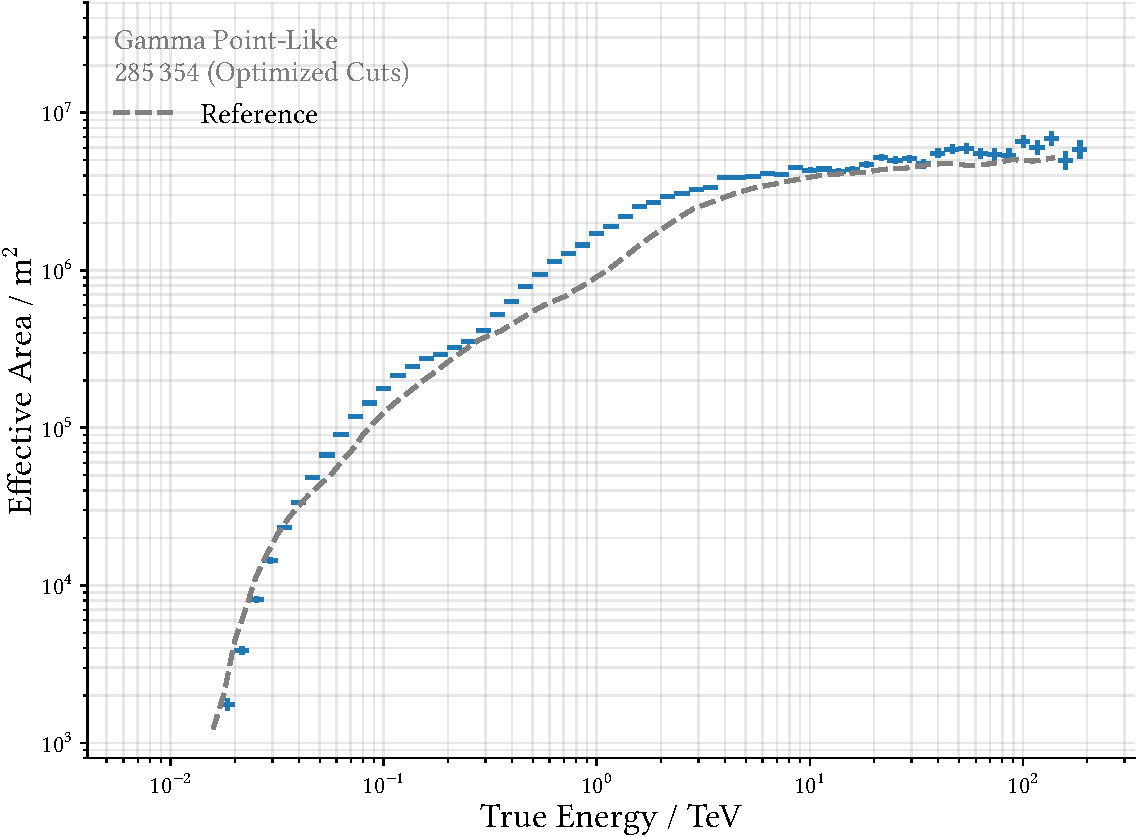
\includegraphics[width=0.6\textwidth]{../analysis/plots/sensitivity/hillas_effective_area.pdf} 
    \caption{Effective area against true event energy for the HillasReconstructor analysis
    with the pointlike gamma events after apllied cuts.
    As no cuts on the low level data have been performed and the high level cuts are relatively
    soft due to the low background event counts, the effective area is bigger at most energies.}
    \label{fig:hillas_area}
\end{figure}

\begin{figure}
    \centering
    \captionsetup{width=0.9\linewidth}
    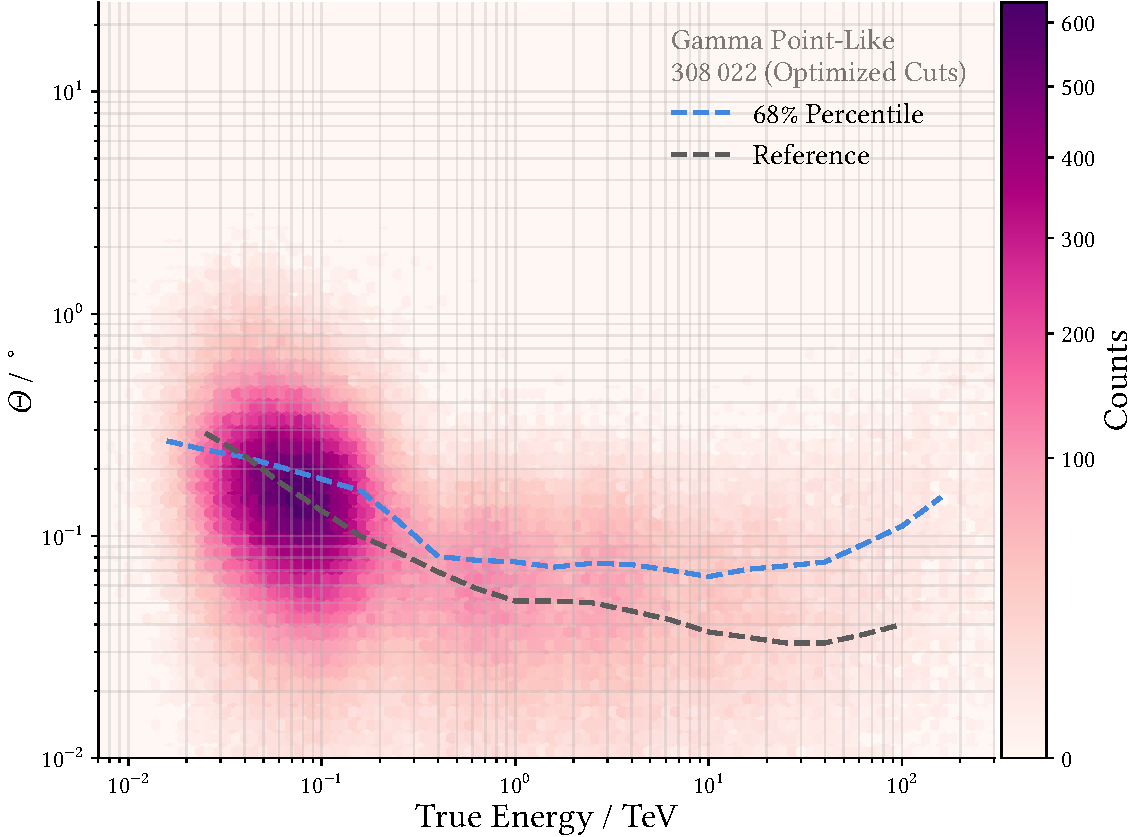
\includegraphics[width=0.6\textwidth]{../analysis/plots/sensitivity/hillas_resolution.pdf} 
    \caption{Angular resolution against true event energy after applied 
    prediction and multiplicity cuts for the HillasReconstructor analysis.
    For better illustration the colorbar has been scaled to account for the
    low event counts at high energies and no $\Theta$ cut is applied.}
    \label{fig:hillas_resol}
\end{figure}

Performing a grid search for the DISP analysis yields very similar cuts
in the prediction threshold and multiplicity (see table \ref{tab:disp_cuts}).
The direction cuts on the other hand are softer for high energies,
the total event counts are then once again comparable.

\newpage
\KOMAoption{paper}{landscape}
\areaset{2\textwidth}{.9\textheight}
\recalctypearea
    \centering
    \begin{tabular}{c c c c c r c c}
        %\hline
        $E_\text{min}$ / \si{\tera\electronvolt} & $E_\text{max}$ / \si{\tera\electronvolt} & $\alpha$ & $\Theta$ & Mult. & Sign. & sig counts & bkg counts \\
        \hline
        \num{0.02} & \num{0.03} & 0.75 & 0.15 & 2 & \num{85.30} & \num{19993.86} (\num{4924}) & \num{192060.04} (\num{466})\\
        \num{0.03} & \num{0.05} & 0.6 & 0.17 & 2 & \num{171.82} & \num{69965.93} (\num{16658}) & \num{562911.14} (\num{1183}) \\
        \num{0.05} & \num{0.08} & 0.6 & 0.17 & 2 & \num{388.16} & \num{200432.42} (\num{46953}) & \num{760783.92} (\num{2001}) \\
        \num{0.08} & \num{0.12} & 0.65 & 0.15 & 2 & \num{495.51} & \num{166607.87} (\num{39931}) & \num{207045.76} (\num{841}) \\
        \num{0.13} & \num{0.20} & 0.7 & 0.11 & 6 & \num{396.09} & \num{56680.18} (\num{14287}) & \num{10013.58} (\num{85}) \\
        \num{0.20} & \num{0.32} & 0.8 & 0.10 & 6 & \num{293.67} & \num{25293.69} (\num{7069}) & \num{499.86} (\num{6}) \\
        \num{0.32} & \num{0.50} & 0.8 & 0.08 & 10 & \num{264.91} & \num{19863.06} (\num{6275}) & \num{84.86} (\num{2}) \\
        \num{0.50} & \num{0.80} & 0.8 & 0.08 & 6 & \num{290.82} & \num{32776.77} (\num{9031}) & \num{46.86} (\num{2}) \\
        \num{0.80} & \num{1.26} & 0.8 & 0.08 & 7 & \num{235.79} & \num{15656.71} (\num{7354}) & \num{39.47} (\num{2}) \\
        \num{1.26} & \num{2.00} & 0.75 & 0.08 & 10 & \num{191.49} & \num{10300.78} (\num{6073}) & \num{17.79} (\num{1}) \\
        \num{2.00} & \num{3.17} & 0.75 & 0.09 & 6 & \num{184.62} & \num{9562.36} (\num{7745}) & \num{12.82} (\num{1}) \\
        \num{3.17} & \num{5.02} & 0.7 & 0.08 & 7 & \num{134.23} & \num{5091.10} (\num{5647}) & \num{18.62} (\num{3}) \\
        \num{5.02} & \num{7.96} & 0.7 & 0.08 & 9 & \num{91.14} & \num{2340.08} (\num{3701}) & \num{6.14} (\num{1}) \\
        \num{7.96} & \num{12.62} & 0.7 & 0.09 & 6 & \num{76.08} & \num{1632.71} (\num{3885}) & \num{4.97} (\num{1}) \\
        \num{12.62} & \num{20.00} & 0.65 & 0.08 & 10 & \num{41.84} & \num{500.16} (\num{1839}) & \num{3.91} (\num{1}) \\
        \num{20.00} & \num{31.70} & 0.6 & 0.1 & 5 & \num{36.38} & \num{379.53} (\num{2176}) & \num{3.54} (\num{1}) \\
        \num{31.70} & \num{50.24} & 0.6 & 0.1 & 2 & \num{23.86} & \num{170.69} (\num{1606}) & \num{5.40} (\num{3}) \\
        \num{50.24} & \num{72.62} & 0.45 & 0.12 & 4 & \num{15.90} & \num{77.76} (\num{1232}) & \num{3.64} (\num{1}) \\
        \num{79.62} & \num{126.19} & 0.45 & 0.11 & 2 & \num{8.36} & \num{24.45} (\num{685}) & \num{3.59} (\num{2}) \\
        \num{126.19} & \num{200.00} & 0 & 0.01 & 2 & \num{0.32} & \num{0.27} (\num{14}) & \num{2.43} (\num{1}) \\
    %\hline
    \end{tabular}
\clearpage
\newpage
% \KOMAoptions{paper=portrait,pagesize}
% \recalctypearea
\normalsetting

The resulting instrument response functions can be seen in figures
\ref{fig:disp_sens}, \ref{fig:disp_area} and \ref{fig:disp_resol}.
At energies up to a few \si{\tera\electronvolt} the effective area is slightly larger, 
for higher energies it falls off.
This is in line with the worse resolution at high energies, that was
previously displayed.
The angular resolution is very much identical, but
the event counts at high energies are lower as also shown by the effective area.

In comparison to the HillasReconstructor analysis, the sensitivity
is slighty improved for event energies under \SI{100}{\giga\electronvolt} and 
worse above.


\begin{figure}
    \centering
    \captionsetup{width=0.9\linewidth}
    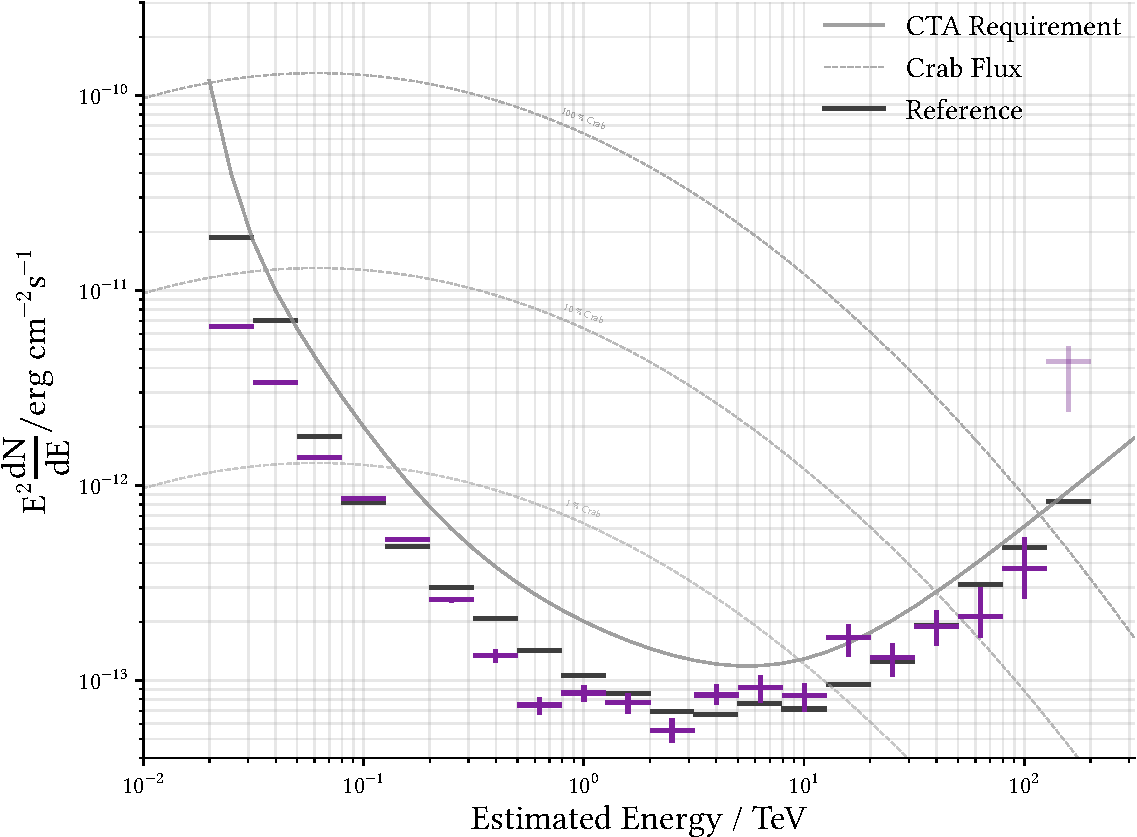
\includegraphics[width=0.6\textwidth]{../analysis/plots/sensitivity/disp_sensitivity.pdf} 
    \caption{Computed sensitivity for the HillasReconstructor analysis against estimated event energy.
    In comparison to the HillasReconstructor analysis, the results at the low energy bins are slightly
    superiour under \SI{100}{\giga\electronvolt} and worse
    above \SI{1}{\tera\electronvolt}.
    Similar conclusions regarding the background statistic and uncertainties
    at high energies can be drawn.}
    \label{fig:disp_sens}
\end{figure}

\begin{figure}
    \centering
    \captionsetup{width=0.9\linewidth}
    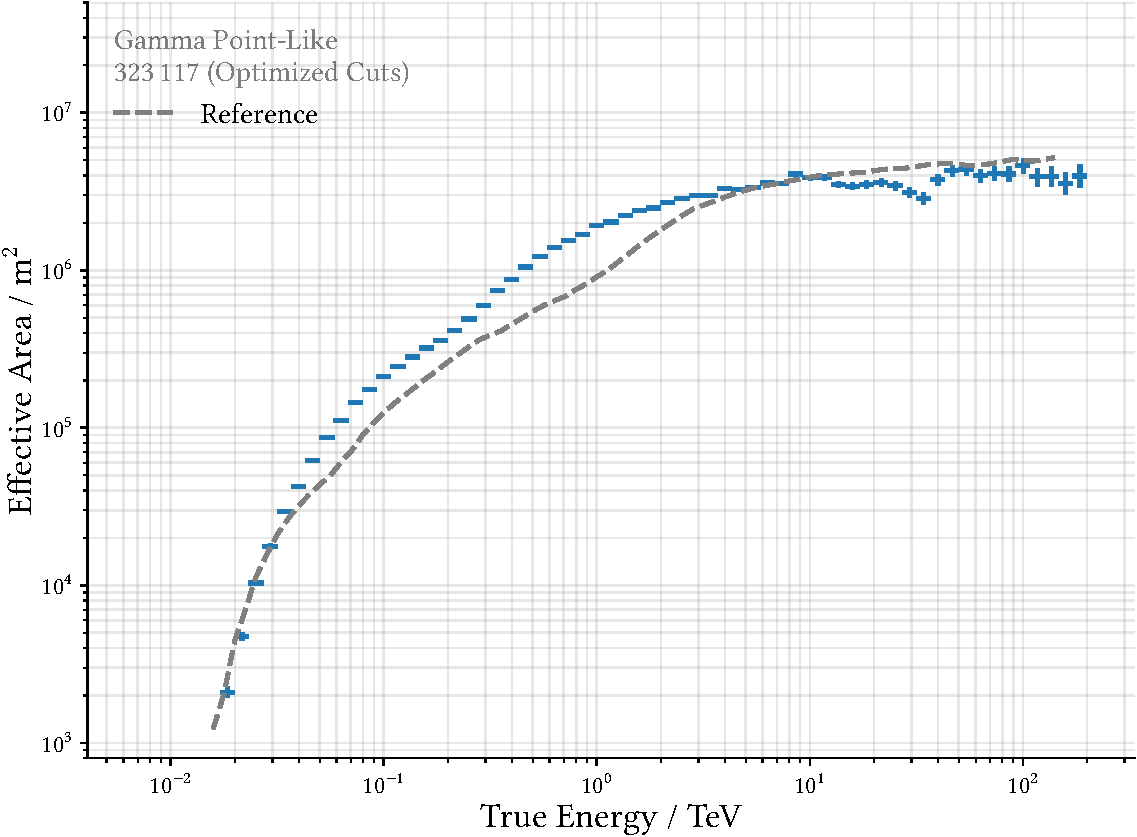
\includegraphics[width=0.6\textwidth]{../analysis/plots/sensitivity/disp_effective_area.pdf} 
    \caption{Effective area against true event energy for the DISP analysis
    with the pointlike gamma events after apllied cuts.
    The effective area is even larger for low and mid energies compared 
    to the previous HillasReconstructor results, but falls short above
    $\SI{10}{\tera\electronvolt}$.}
    \label{fig:disp_area}
\end{figure}

\begin{figure}
    \centering
    \captionsetup{width=0.9\linewidth}
    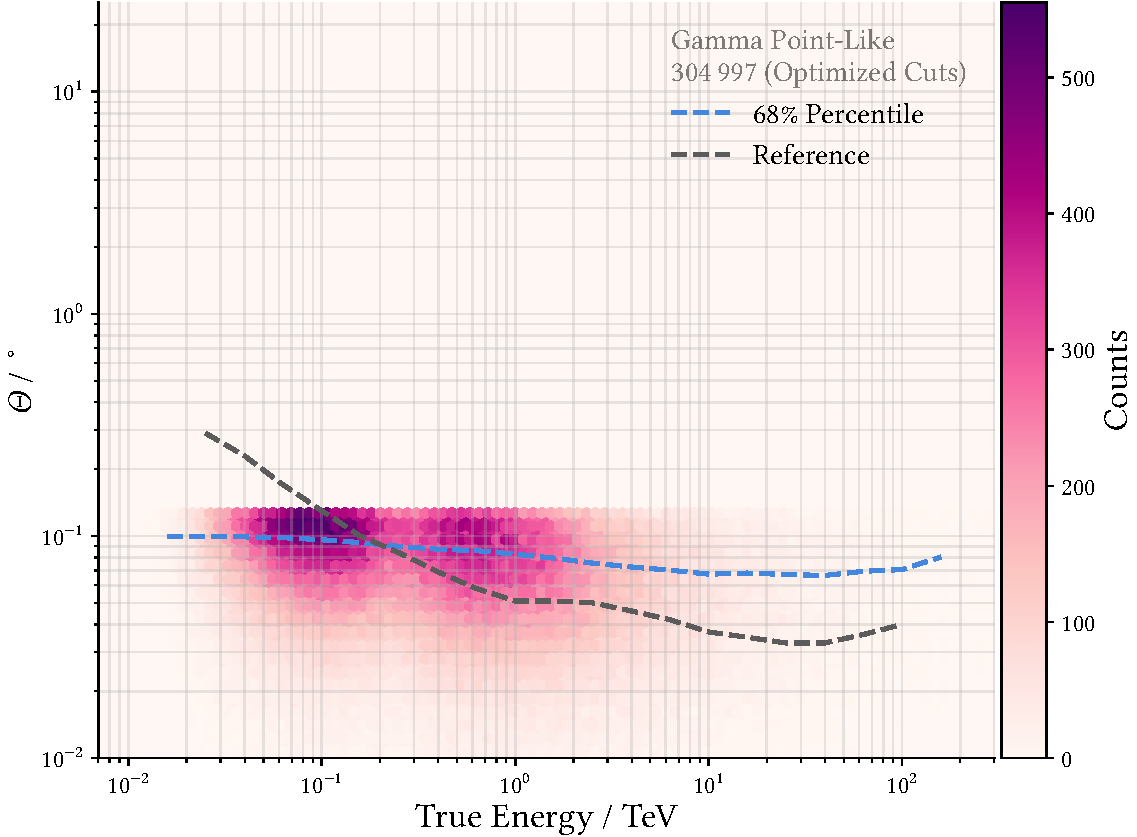
\includegraphics[width=0.6\textwidth]{../analysis/plots/sensitivity/disp_resolution.pdf} 
    \caption{Angular resolution against true event energy after applied 
    prediction and multiplicity cuts for the DISP analysis.
    For better illustration the colorbar has been scaled to account for the
    low event counts at high energies and no $\Theta$ cut is applied.}
    \label{fig:disp_resol}
\end{figure}